We will start by comparing the trainings with the following inputs: 
\begin{itemize} [itemsep=0.1em]
    \item 4 jets 
    \item 4 jets with a fifth jet as global input (therefore this fifth jet is not used for the pairing but it adds information about the kinematics of the system)
    \item 5 jets as inputs
\end{itemize}

In Figures \ref{fig: val acc 4j/5j/4j5g} and \ref{fig: eff 4j/5j/4j5g} we compare these trainings according to the validation accuracy and the efficiency of the paring as a function of the di-higgs mass.

\begin{figure}[hbt]
    \centering
    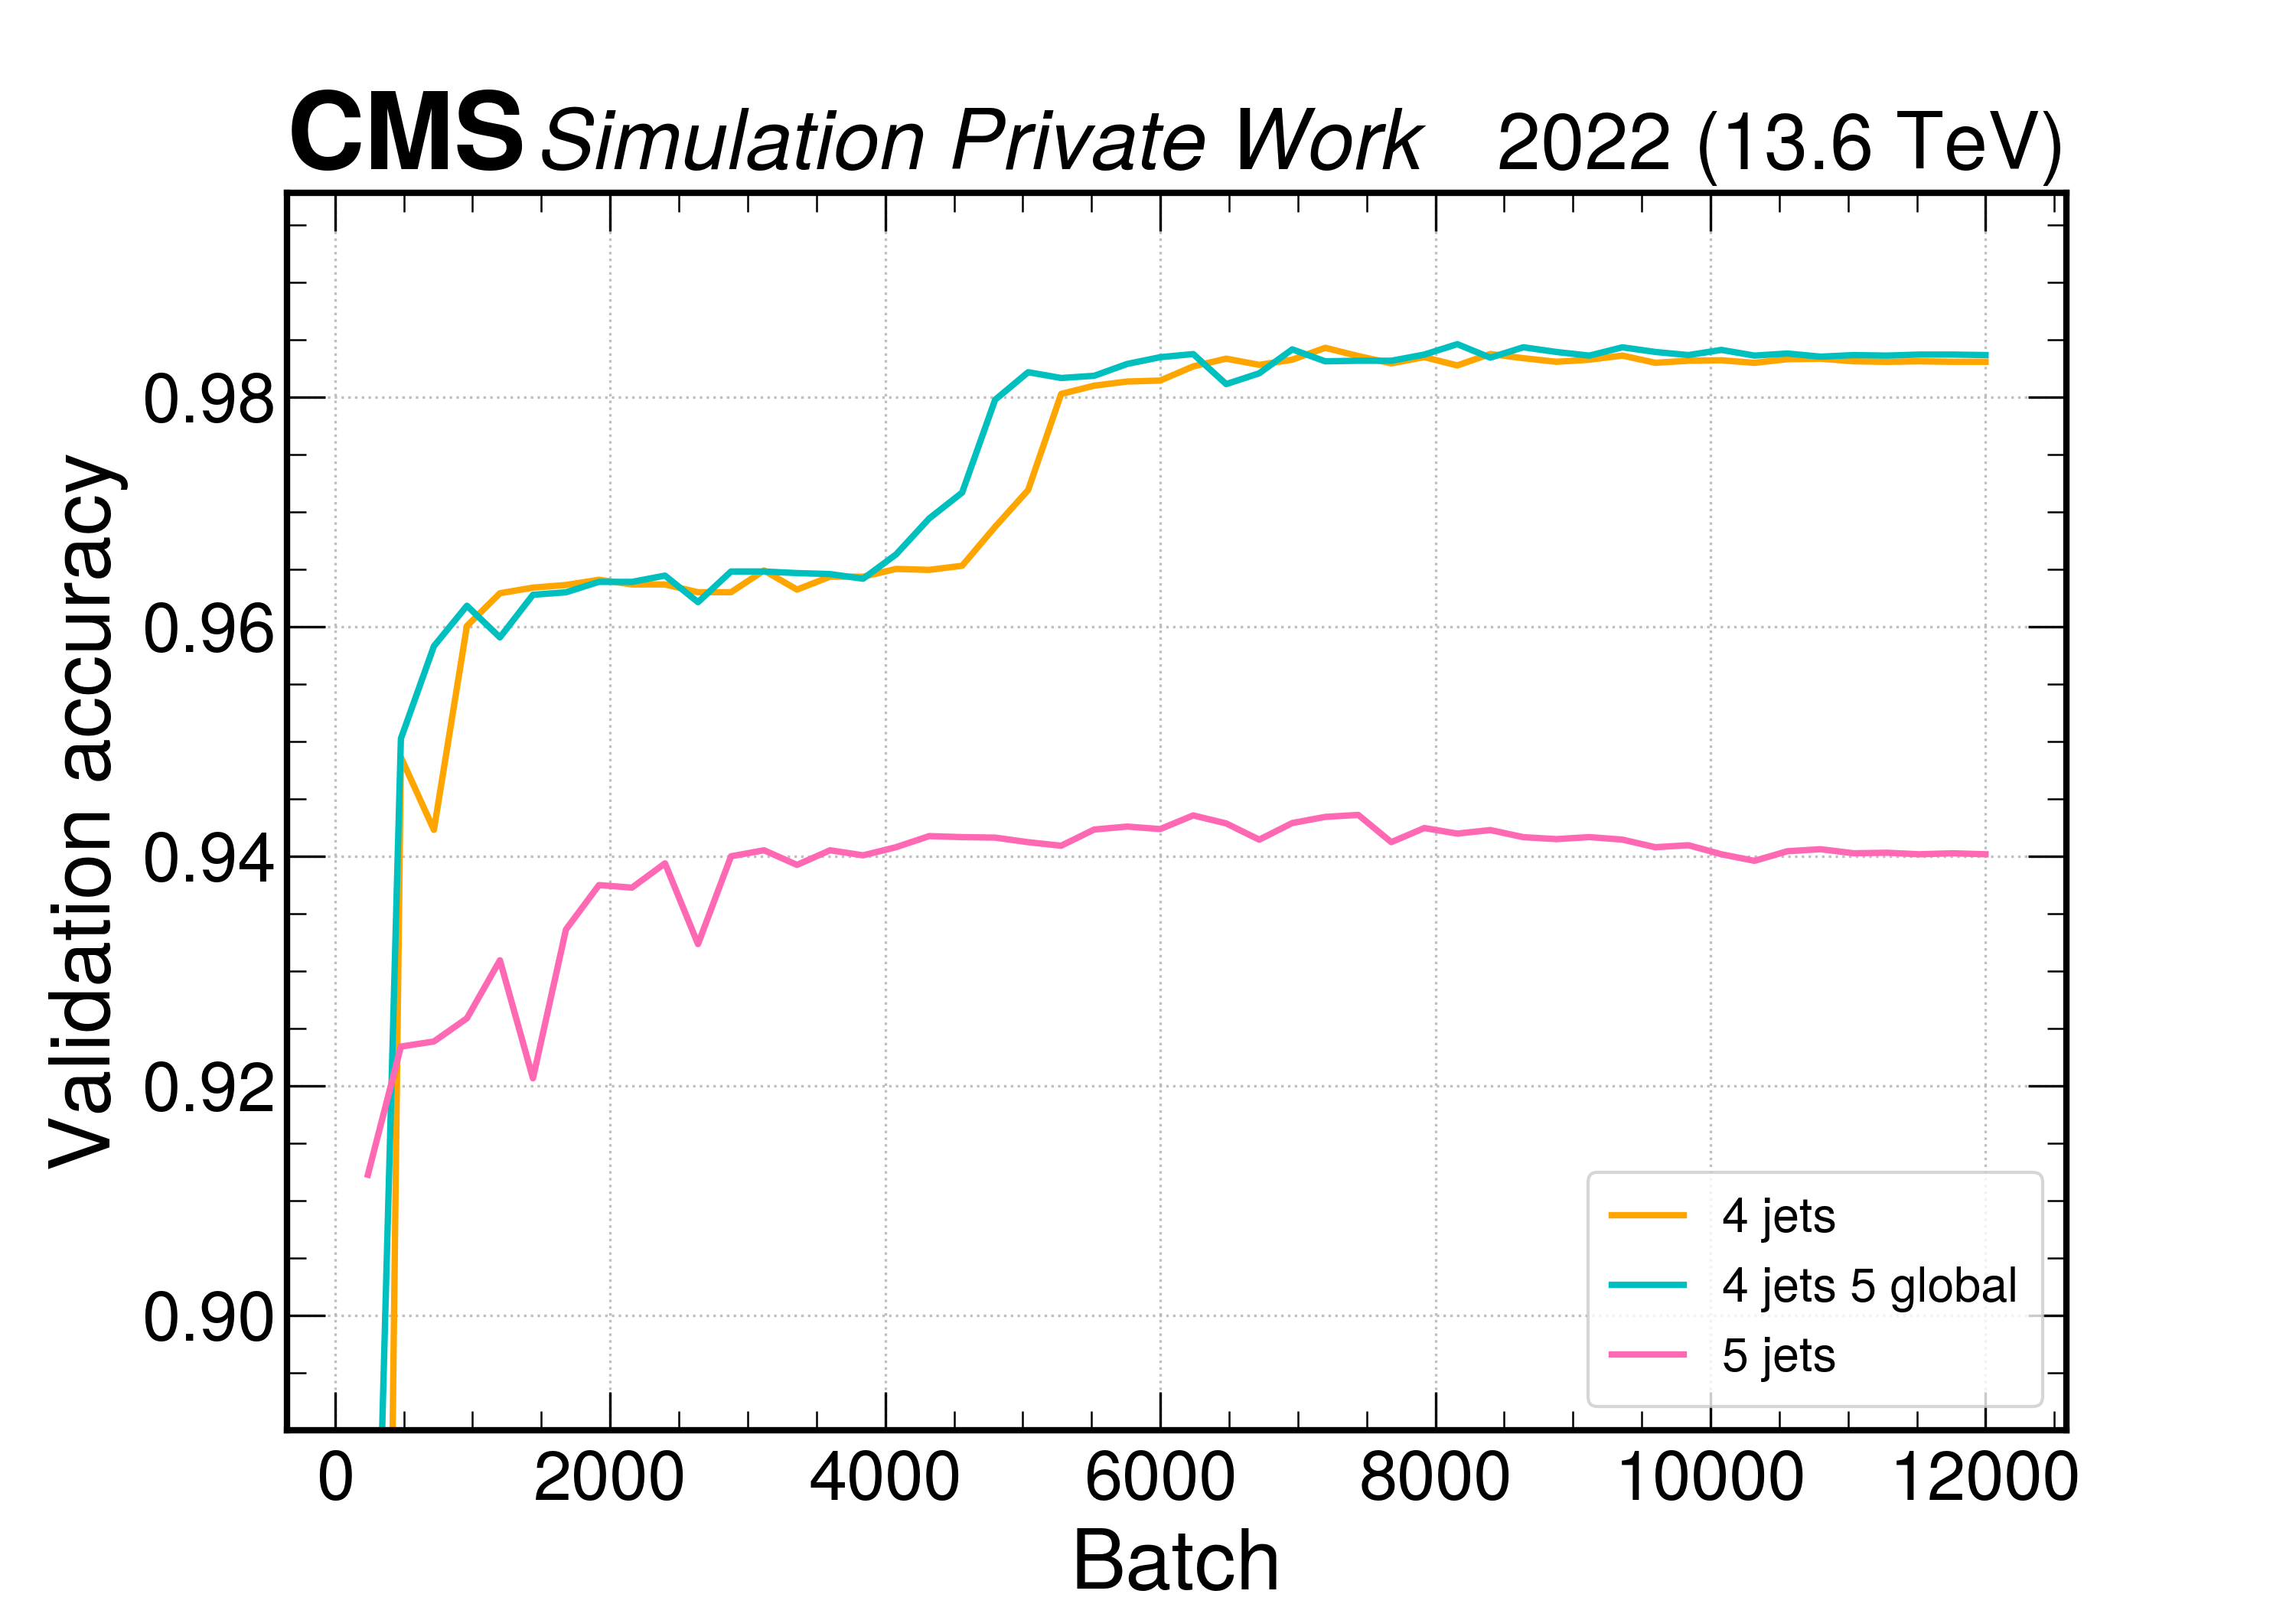
\includegraphics[width=0.5\linewidth]{Images/6.Improving/Imput Comparisons/VA 4 vs 5 vs 4j5g.png}
    \caption{Validation accuracy of the trainings with 4, 5 jets and 4 jets with a 5th jet as global input}
    \label{fig: val acc 4j/5j/4j5g}
\end{figure}


\begin{figure}[hbt]
    \centering
    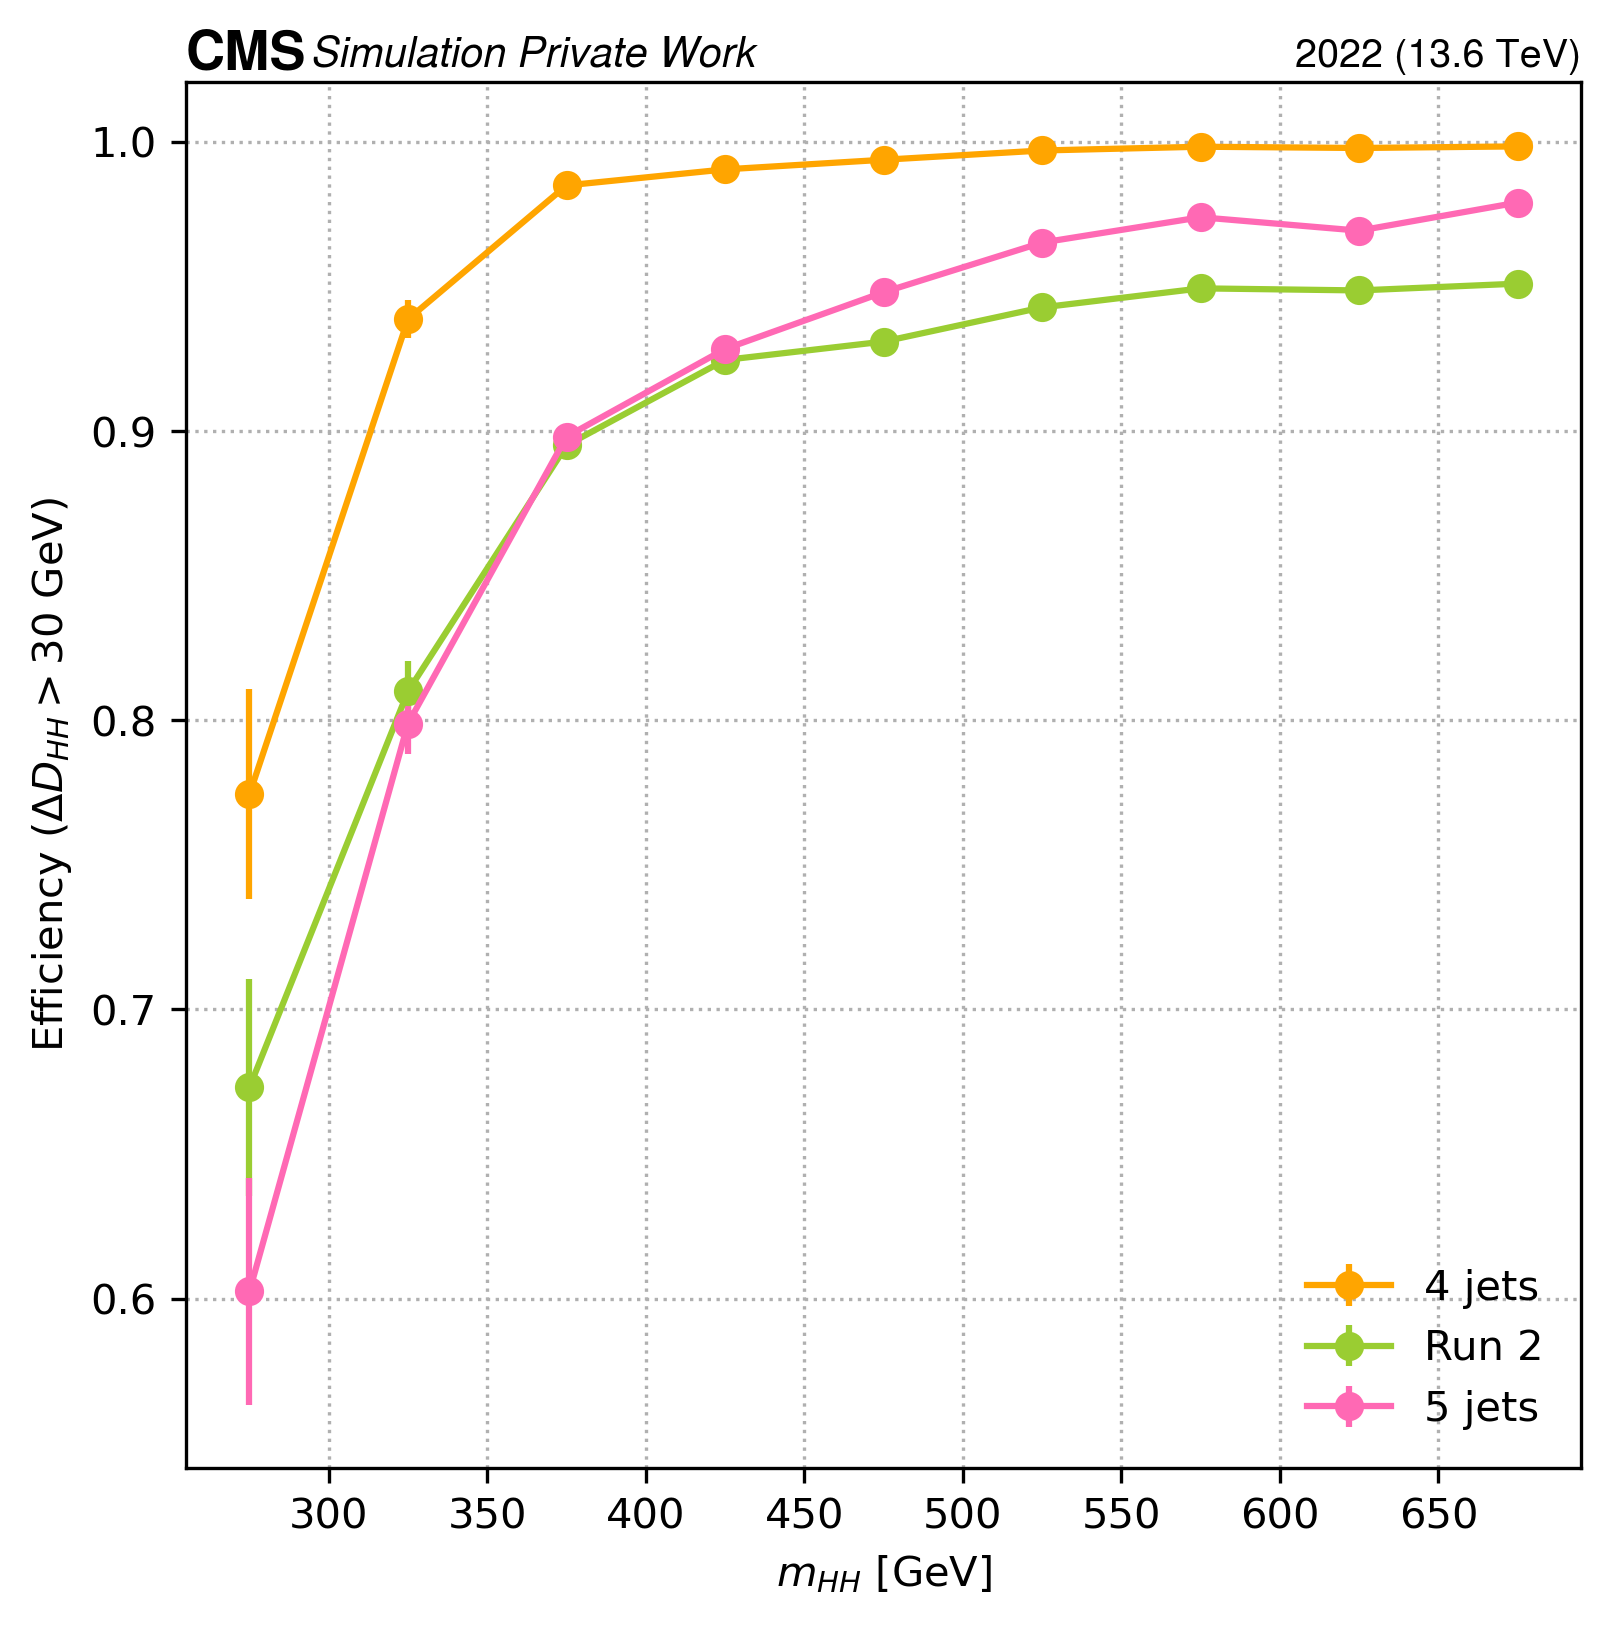
\includegraphics[width=0.5\linewidth]{Images/6.Improving/Imput Comparisons/Eff 4 vs 5 vs R2.png}
    \caption{Pairing efficiency}
    \label{fig: eff 4j/5j/4j5g}
\end{figure}


In Figure \ref{fig:tot eff 4j/5j/4j5g} it becomes clear that when comparing the total effciency, the best trainings are the ones using 5 jets as inputs or 4 jets with a 5th jet as global input. For rest of the report we will only be considering these inputs. We will refer to 4 jets to the trainings done with 4 jets with a 5th global jet as input.

\begin{figure}[hbt]
    \centering
    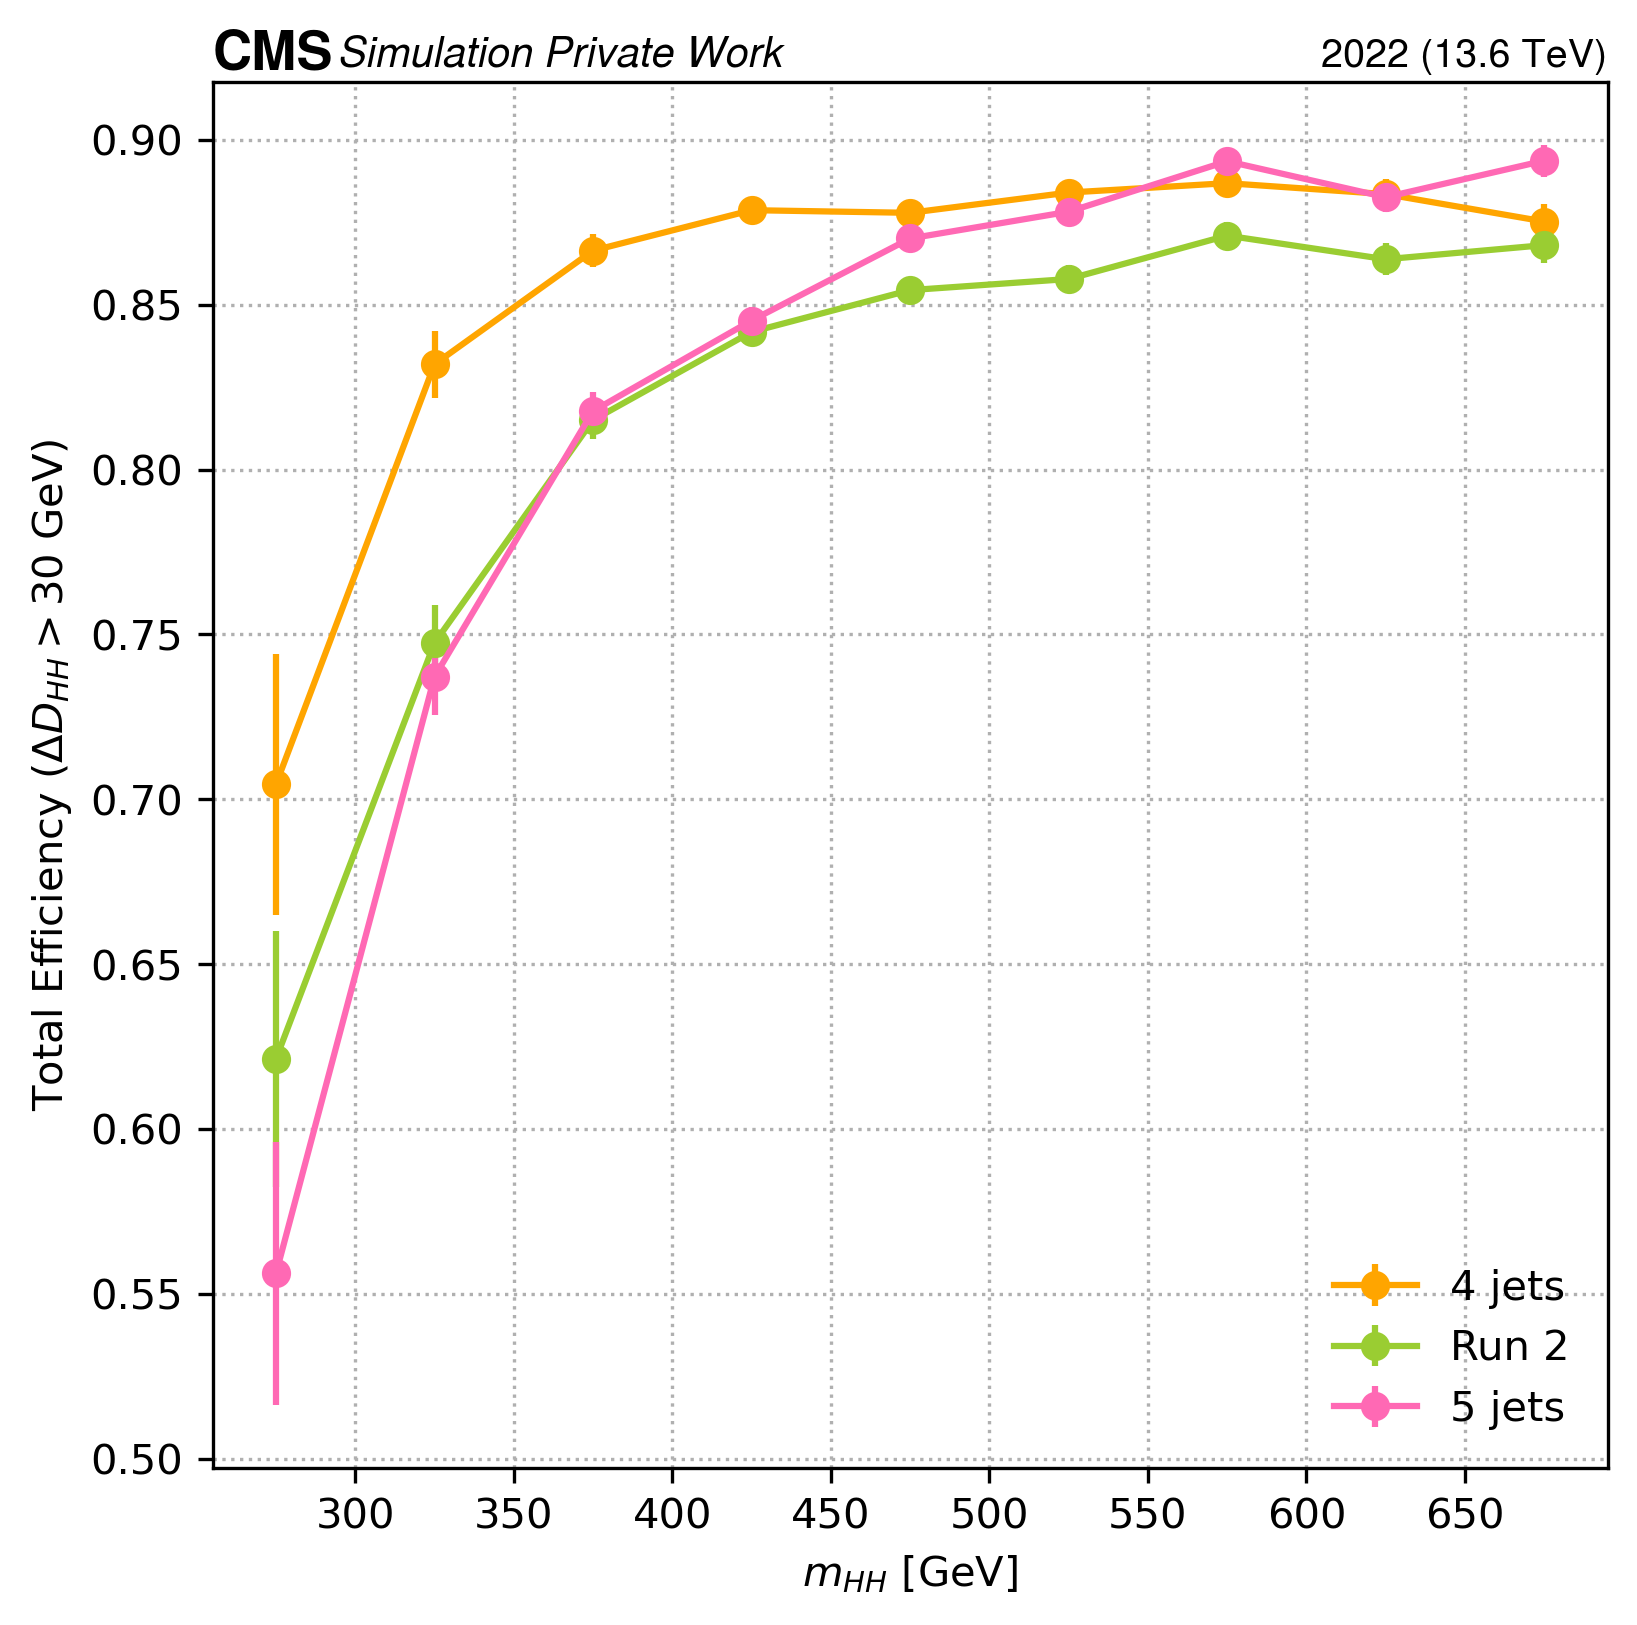
\includegraphics[width=0.5\linewidth]{Images/6.Improving/Imput Comparisons/Tot Eff 4vs 5 vs R2.png}
    \caption{Total pairing effciency}
    \label{fig:tot eff 4j/5j/4j5g}
\end{figure}

As a next step we will be comparing different configurations within the trainings using 5 jets as inputs or 4 jets with a fifth global. 